\namedsubsection{FPGA}{Pasat}

A FPGA (field-programmable gate array) is an semiconductor device which is has a matrix of CLBs (configurable logic blocks) connected through programmable interconnects. One main advantage of FPGAs is that the can be preprogrammed after they are manufactured in order to fit desired functionalities and requirements, such as the ones required by our team's project. Amazing projects have also been realized with this processor on a FPGA, such as advanced real traffic light controller \cite{traffic_light}.

The two devices we are using, the FPGA and the microcontroller, are two very different devices. The microcontroller has the chip already designed. The programmer simply writes the software in C or C++, then it is compiled into a hex file that is loaded on the microcontroller. The program is stored in the flash memory until is is replaced or erased.

FPGAs are different in this sense. The circuit is completely designed by the programmer. The processor must be created and can be as simple as an and gate or can be our Cortex M0+. HDL is used to write the design, which is then synthesized into a bit file which configures the FPGA. One small problem with this is the fact that it stores the configuration in the RAM, so once the power is gone, the configuration is lost.

The board used for this project is the Xilinx Digilent Nexys4, which can be seen in figure \ref{fig:nexys4} above. It is based on the Artix-7 that has the lowest power consumption at 28nm and is optimized to give the design the highest performance \cite{cortexm0onnexys4}. Implementations were also successful on low end FPGAs. We chose this board because it is a large, high-capacity FPGA board that would be sufficient for our project. Another reason is the fact that is has several built in peripherals, such as accelerometer, which would be useful for the exercise detection. 

\begin{figure}
\centering
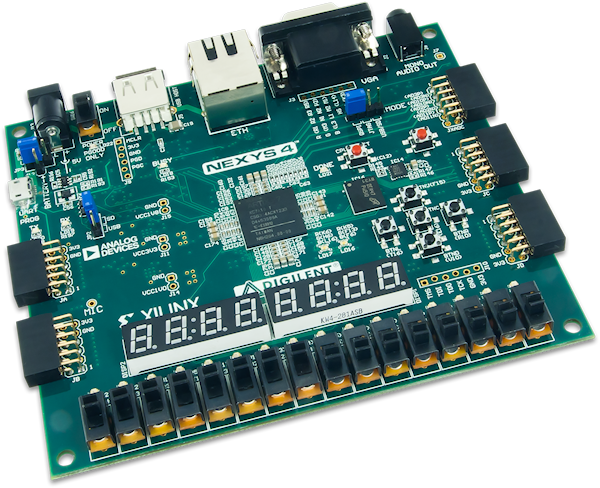
\includegraphics[scale=0.7]{figures/nexys4.PNG}
\caption{Xilinx Digilent Nexys4 \label{fig:nexys4}}
\end{figure}

Next,the implementation of the Cortex M0 DesignStart on the FPGA board will be discussed. The system will have a Cortex-M0\_DS processor, a preloaded memory with a program that fetches constants from a memory at regular intervals, a reset and a pattern detector attached to the bus so when a specific pattern appears on the data bus, the LED turns on and when another patters appears it will turn off. The Cortex-M0\_DS  includes only the processor a non-synthesizable testbench. Other parts will need to be implemented in order to create an synthesizable system: a software executable image, a memory holding the program, a system clock, a detector module for the command LED and a reset synchronizer. This section will be divided into: software development and simulation, system implementation and functional simulation. All of these sections will be discussed in detail in what follows.

